\chapter{Fachliches Umfeld}\label{chp:fachlichesumfeld}

%#######################################################################################
%#######################################################################################
\section{TESTONA}\label{sec:Testona} 
\paragraph{}

Mit TESTONA wird dem Tester ein Tool angeboten, um signifikante Testszenarien und -umfänge strukturiert zu bestimmen. Mit das Programm können komplette Testspezifikationen schnell und einfach generiert werden und überflüssige Testfälle vermieden werden. Bei Bedarf gibt es die Möglichkeit automatische generierte Testspezifikationen und Testfälle bequem mit Anforderungen durch Add-Ons an Standard-Werkzeugen zu verlinken (siehe \ref{sec:DOORS}). Somit werden robuste Schnittstellen für ein komfortables Anforderungs- und Testmanagement erzeugt. Ein sehr wichtiger Aspekt von TESTONA ist, dass es Branchen-unabhängig ist. Dass heißt ein Tester kann TESTONA im jedem Fachgebiet benutzen, nicht nur bei Software- oder Funktionstests.\\

Mehr zu Testfällen und die Arbeitsweise dieses Programms werden in den nächsten Kapiteln erläutert, wie zum Beispiel die anerkannte Klassifikationsbaum-Methode.



%#######################################################################################
\subsection{Klassifikationsbaum-Methode}\label{ssec:KM}
\paragraph{}
In 1993 entwickelten K. Grimm und M. Grochtmann die Klassifikationsbaum-Methode zur Ermittlung funktionaler Backbox-Tests im Bereich von eingebetteter Software. Die Methode wurde im Forschungslabor von Daimler-Benz in Berlin als Weiterentwicklung der Category-Partition Method (CPM) erforscht. Gegenüber CPM hat die Klassifikationsbaum-Methode eine graphische Baum-Darstellung und hierarchische Verfeinerungen für implizite Abhängigkeiten. Als Werkzeug wurde der \glqq Classification Tree Editor\grqq~ (CTE) \footnote{Entwickelt von Grochtmann und Wegener\cite{TestCaseDesign}. Bei Berner  \& Mattner aus rechtlichen Gründen zu TESTONA umbenannt} programmiert und unterstützt Partitionierung und Testfallgenerierung. Das Werkzeug von CPM konnte nur Testfälle generieren ohne Bestimmung der Testaspekte\cite{ClassificationTrees}.

 Diese Methode besteht aus zwei wichtige Schritten:
\begin{itemize}
\item Bestimmung der Klassifikationen (testrelevante Aspekte) und Klassen (mögliche Ausprägungen).
\item Erzeugung von Testfällen aus Kombinationen von unterschiedlichen Klassen für alle Klassifikationen
\end{itemize}

Ansatzpunkt sind die Funktionale Anforderungen (siehe \ref{sec:DOORS}) eines zu testendes Objekt. Um die Testfälle zu definieren und erzeugen, folgt die Methode das Prinzip des kombinatorischen Testentwurfs \cite{KlassifikationsbaumMethode}. Dieses Prinzip hilft bei der Detektierung von Fehler in frühe Schritte des Testvorgangs. Nicht jeder einzelne Parameter steuert ein Fehler bei, eher werden Fehler durch die Interaktion verschiedene Parameter verursacht. Betrachten wir ein einfaches Beispiel, indem ein Programm auf Windows oder Linux laufen soll, unter Verwendung eines AMD oder Intel Prozessors und mit Unterstützung des IPv4 oder IPv6 Protokolls. Das ergibt intuitiv acht verschiedene Testfälle ($2^{3} = 8$ Möglichkeiten, siehe Abbildung \ref{ttn.no_kombi}).\\

\begin{figure}[h]
  \begin{center}
    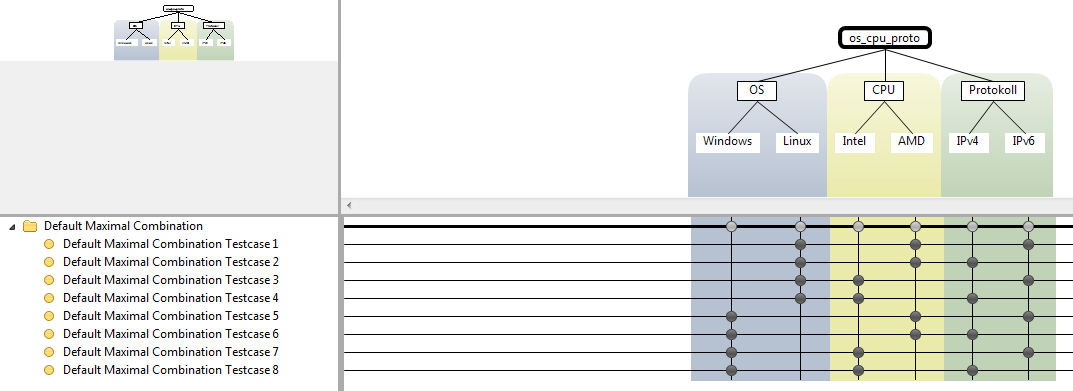
\includegraphics[scale=0.5]{os_cpu_proto_max_kombinatorik.png}
  		  \caption{Baum und Testfälle ohne Kombinatorik}
     \label{ttn.no_kombi}
  \end{center}
\end{figure}


Verwenden wir dafür der kombinatorische Testentwurf \glqq paarweise Kombination\grqq~ (in Testona: \textit{pairwise}(OS, CPU, Protokoll) ), hätten wir nur vier Testfälle (siehe Tabelle \ref{table:4TestCases}). Durch diese Methode werden alle Kombinationspaare der Parameter mindestens durch ein Testfall gedeckt\cite{CombinatorialSoftTesting}.\\

\begin{table}[h]


\begin{center}
	\begin{tabular}{|r||c|c|c|}
	 \hline
	 No. &OS &CPU &Protokoll\\
	 \hline
	 1. &Linux &AMD &IPv6\\
	 \hline
	 4. &Linux &Intel &IPv4\\
	 \hline
	 5. &Windows &AMD &IPv6\\
	 \hline
	 8. &Windows &Intel &IPv4\\
	 \hline
	\end{tabular}
	
	\caption{Testfälle mittels paarweise Kombinatorik}
	\label{table:4TestCases}
\end{center}

\end{table}


%\begin{figure}[h]
%  \begin{center}
%    \includegraphics[scale=0.35]{a.png}
%  		  \caption{Testfälle aller Möglichkeiten}
%     \label{ttn.gruen}
%  \end{center}
%\end{figure}

Die Effizienz von diesen einfachen kombinatorischen Entwurf ist bei komplexeren System zu sehen. Hat ein System $20$ verschiedene Schalter und jeder Schalter $10$ verschiedene Einstellungen, so gibt es $10^{20}$ verschiedene Kombinationen. Durch Anwendung der paarweise Kombination muss der Tester nur 180 Testfälle betrachten.\\

Ein Experiment hat gezeigt, dass durch die Verwendung von die paarweise Kombinatorik die gleichen oder meistens mehrere Fehler entdeckt wurden, als mit manuelle Testauswahl\footnote{Basierend auf funktionelle und technische Anforderungen, Use-Cases}. Paarweise Kombinatorik ist am meisten verbreitet, aber man kann durchaus auch Drei-Wege-Kombinatorik verwenden. TESTONA implementiert standardmäßig Minimalabdeckung, Paarweise-, Drei-Wege- und N-Kombinatorik (wo N die maximale Anzahl an möglichen Parameter im Klassifikationsbaum ist, auch vollständige Kombinatorik genannt)\cite{CombinatorialSoftTesting}.\\




%#######################################################################################
\subsection{Testfälle und Testfallgenerierung}
\paragraph{}
%Reduzierte Testaufwände durch einheitlichen und domänenunabhängigen

%Einsatz in allen Testphasen
%Kostensenkung durch automatisierte Testfallgenerierung
%Präzise Bestimmung der Testtiefe
%Messbare Beurteilung der Testabdeckung


Unter ein Testfall ist zu verstehen, die Beschreibung eines elementaren Zustands eines Testobjekts. Hierfür werden Eingangsdaten benötigt (Parameterwerte, Vorbedingungen) und ein erwarteter Folgezustand. Mit TESTONA werden Testfälle definiert für eine vereinbarte Testspezifikation. Laut IEEE 829 ist unter Testspezifikation die Durchführung von:

\begin{itemize}
\item\textbf{ Testentwurfsspezifikation}: verfeinerte Beschreibung der Vorgehensweise für das Testen einer Software
\item \textbf{Testfallspezifikation}: dokumentiert die zu benutzenden Eingabewerte und erwarteten Ausgabewerte
\item \textbf{Testablaufspezifikation}: Beschreibung alles Schritte zur Durchführung der spezifizierten Testfälle.
\end{itemize}

zu verstehen. Da TESTONA in allen Testphasen einsetzbar ist, kann effizient die Arbeitszeit reduziert werden. Dazu hilft auch die automatische Testfallgenerierung und die verschiedene kombinatorische Möglichkeiten (siehe \ref{ssec:KM}) . Somit kann der Tester ein besseren Zeitplan erzeugen und die Arbeitskräfte zielbewusst an der Ausführung und Auswertung der Testfälle beschäftigen.\\

Allgemein wird ein Test laut das ISTQB-Glossar\footnote{International Software Testing Qualification Board} folgendermaßen definiert:

\begin{center}
\textit{
Der Prozess, der aus allen Aktivitäten des Lebenszyklus besteht (sowohl statisch als auch dynamisch), die sich mit der Planung, Vorbereitung und Bewertung einer Softwareprodukts und dazugehörige Arbeitsergebnisse befassen. Ziel des Prozesses ist sicherzustellen, dass diese allen festgelegten Anforderungen genügen, dass sie ihren Zweck erfüllen und etwaige Fehlerzustände zu finden.}\cite{SoftwareTestEmbSys}\\

\end{center}

Anhand der generierten Testfälle und die Benutzung von  kombinatorische Möglichkeiten kann der Tester einfach eine präzise Testtiefe erreichen. Die Testtiefe wird anhand der Durchführung einer Risikoanalyse vereinbart und die Auswertung des Kritikalitätsstufe (sehr hoch, hoch, mittel und tief) des Systems. Das soll heißen, dass die Testtiefe für ein Flugzeug (Kritikalitätsstufe = sehr hoch\footnote{Das Fehlverhalten kann zu Verlust von Menschenleben führen, die Existen des Unternehmens gefährden}) viel höher und genauer ist, als die Kompatibilität eines Bildschirmes mit ein Graphiktreiber (Kritikalitätsstufe = tief\footnote{Das Fehlverhalten kann zu geringen materiellen oder immateriellen Schäden fuhren}).\\

Anhand der Risikoanalyse und die Kritikalitätsstufe wird auch eine vereinbarte Testabdeckung und Testfallermittlungsverfahren erreicht. Im Fall vom Flugzeug wird eine Kombination von White und Blackbox-Methoden mit sehr hoher Testtiefe ausgeführt. Dagegen im Fall vom Bildschirm wird intuitives Testen mit geringer Testtiefe angewendet.\cite{ApplicationEngineering}

%#######################################################################################
%#######################################################################################
\subsection{Abhängigskeitsregeln}
\paragraph{}

Abhängigkeitsregeln werden vereinbart um überflüssige Testfälle zu vermeiden, bzw. um Vorbedingungen für bestimmte Testszenarien festzulegen. Abhängigkeitsregeln werden Mithilfe von boolische Algebra definiert wie folgende Abbildung \ref{ttn.depencyRules}zeigt:

\begin{figure}[h!]
  \begin{center}
    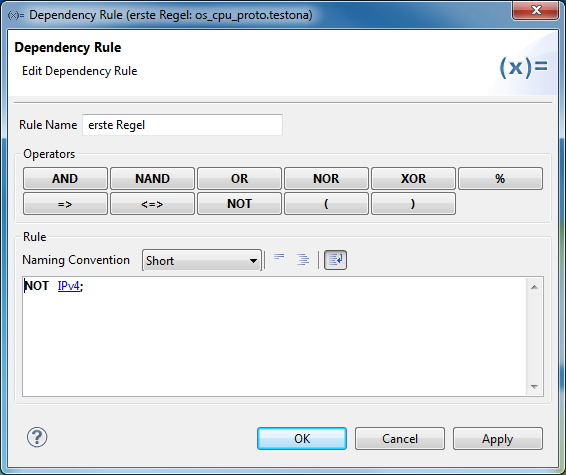
\includegraphics[scale=0.5]{dependency_rules_2.png}
  		  \caption{Abhängigkeitsregeln Bearbeitung}
     \label{ttn.depencyRulesEdit}
  \end{center}
\end{figure}

Boolesche Operatoren:\\

\begin{tabular}{ll}
AND &: Konjunktion\\
NAND &: negierte Konjunktion\\
OR &: Disjunktion\\
NOR &: negierte Disjunktion\\
XOR &: ausschließende Disjunktion\\
\% &: \glqq don't care\grqq~ Operator\\
=> &: vom A folgt B\\
<=> &: A ist gleichwertig wie B\\
NOT &: Negation\\
\end{tabular}

Durch die Verwendung diese Operatoren werden wie folgt Abhängigkeitsregeln definiert:

\begin{figure}[h]
  \begin{center}
    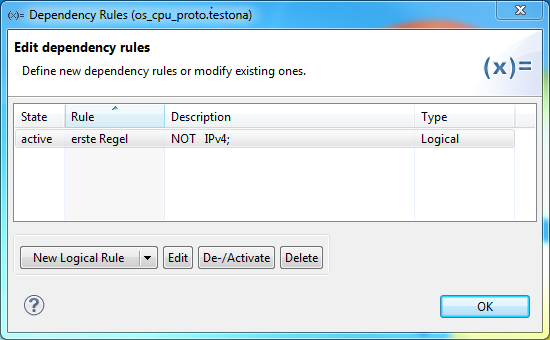
\includegraphics[scale=0.5]{dependency_rules.png}
  		  \caption{Abhängigkeitsregeln Übersicht}
     \label{ttn.depencyRules}
  \end{center}
\end{figure}

Nemmen wir das Beispiel wahr, so will der Tester die Klasse \glqq IPv4\grqq~ für diese Tests ignorieren. Also werden nur Testfälle erzeugt, wo dieser Parameter nicht vorkommt.


\begin{figure}[h]
  \begin{center}
    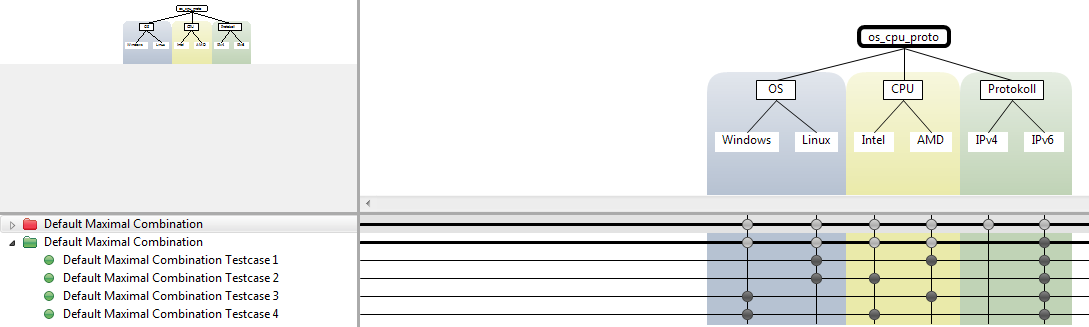
\includegraphics[scale=0.5]{dependency_rules_noParam.png}
  		  \caption{Testfälle mit Anwendung der Abhängigkeitsregeln aus \ref{ttn.depencyRulesEdit} und \ref{ttn.depencyRules}}
     \label{ttn.depencyRules}
  \end{center}
\end{figure}

In diesen einfachen Beispiel wird nur ein Parameter ignoriert, aber durch die Abhängigkeitsregeln kann der Tester durchaus komplexere Fälle einleiten. Es kann die Reaktion eines Systems getestet werden, wo die Spannung sich in einem niedrigen Bereich befindet. Es soll die Spannung einer Batterie geprüft werden, wenn ein Lichtschalter bedient wird. So ein Fall wird geprüft, indem verschiedene Regeln angelegt werden, die folgendermaßen aussehen:

\begin{center}
\textit{Lichtschalter1 XOR Lichtschalter2}\\
\textit{NOT > 5V}
\end{center}

Mit diesen Regeln, werden nur Testfälle betrachtet, wo die Spannung der Batterie kleiner als $5V$ ist, und ein der beiden Lichtschalter betätigt wird.





%#######################################################################################
%#######################################################################################
\newpage
\section{IBM Rational DOORS}\label{sec:DOORS}
\paragraph{}
%kopplung zwischen testona und doors, parameter der anforderungen

%Anbindung an gängige Werkzeuge im Entwicklungs- und Testprozess
%Umfassende Unterstützung des Requirements Tracing

Quality Systems \& Software (QSS) hat am Anfang der 90er Jahre DOORS (Dynamic Object Oriented Requirements System) entwickelt. Die Firma Telelogic kaufte im Jahr 2000 QSS, die wiederum 2008 von IBM übernommen wurde. DOORS ist eine Anforderungsmanagement Software und ermöglicht die Verwaltung und strukturierte Aufzeichnung von Anforderungen (als Objekte). Durch eine tabellarische Ansicht der Anforderungen können geordnet die Anforderungen und die zugehörige Eingenschaften abgelesen werden. Als Eingenschaften sind eine eindeutige Identifikationsnummer, sowie vom Benutzer ausgewählte Attribute.\\


\begin{figure}[h]
  \begin{center}
    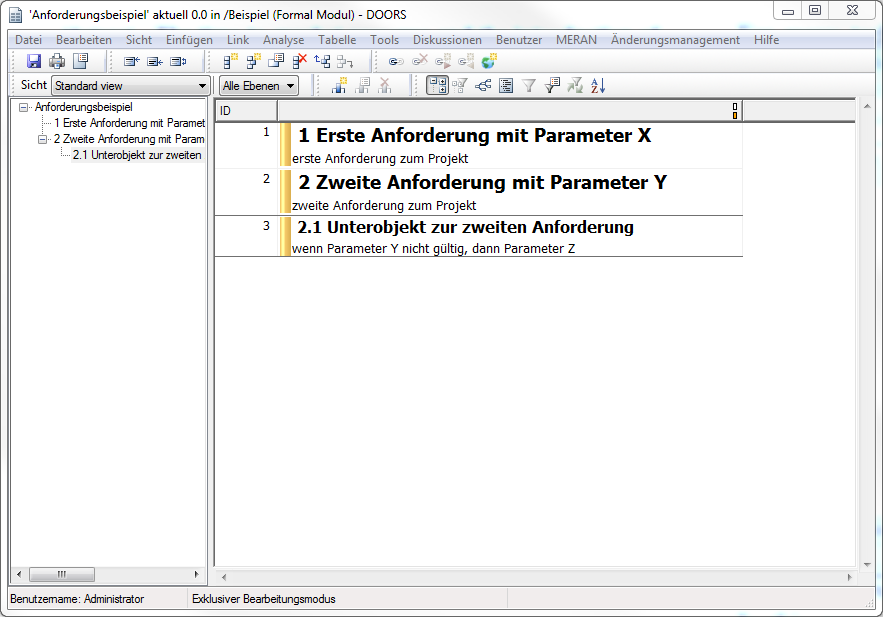
\includegraphics[scale=0.3]{doorsTable.png}
  		  \caption{Beispiel einer Tabelle in DOORS}
     \label{doors.bespiel}
  \end{center}
\end{figure}


In DOORS heißt eine Tabelle \glqq Modul\grqq~ , jede Zeile innerhalb eines Moduls nennt sich \glqq Object\grqq~ und die Spalten für jedes Object bezeichnet man als \glqq Attribut\grqq~. Ein Object kann Unterobjekte besitzen, indem Alternativen und weitere Anforderungen beschrieben werden (siehe Abbildung \ref{doors.bespiel}).

Um Anforderungen im Laufe des Projektes zu verfolgen (Tracing), können Anforderungen miteinander verlinkt werden. DOORS basiert sich auf eine Client - Server Anwendung mit einer proprietären Datenbank. \\
\\
Es werden auch Schnittstellen für den Datenaustausch zur Verfügung gestellt (Testmanagement-, Modellierungs- und Changemanagementwerkzeugen) dank der Unterstützung von RIF (Requirements Interchange Format). Durch die Skriptsprache \glqq DXL\grqq~ (DOORS eXtention Language) erhält TESTONA zugriff auf die gespeicherten Anforderungen in DOORS (durch die Ausführung von Skripts). \cite{Doors} \cite{Anforderungsmanagement}\\

Um diese Aufgabe kümmert sich der TESTONA Plug-in \textit{com.berner\_mattner.testona.requirements.doors}. Dieses Plug-in beinhaltet den Java-Code für TESTONA, sowie die \textit{dxl} Scripts für DOORS.


%#######################################################################################
%#######################################################################################
\newpage
\section{Variantenmanagement}\label{sec:VarManag}
\paragraph{}

Variantenmanagement, wie das Wort schon verrät, behandelt verschiedene Varianten eines Produktes. Leider gibt es oft Verwechslungen mit Feature Management. Um es besser zu unterscheiden soll folgendes Beispiel betrachtet werden. Ein Wagen kann in verschiedene Modelle gebaut werden: Coup\'{e}, Limousine, Cabrio. Alle sind Wagen und haben alle grobe Eigenschaften eines Wagens (4 Räder, Personenkraftwagen, etc), aber unterscheiden sich durch die Anzahl der Passagiere oder die Größe des Wagens. Diese sind Varianten eines Wagens der in verschiedene Modelle angeboten wird. \cite{VarMan1} \\

Hier wird klar, dass durch die steigenden Produktkomplexität bzw. -vielfalt die Identifikationsmerkmale zur Definition einer Produktvariante immer schwieriger zu vereinbaren sind. Für diese Masterarbeit ist eher wichtig, Identifikationsmerkmale zu definieren, die dazu führen, dass die Tests oder der Testablauf eines Produktes sich ändert (mehrere Testfälle sind nötig, neue Parameterwerte). Das heißt, wenn ein Wagen als Coup\'{e} gebaut wird und danach als Cabrio angeboten wird, müssen (unter anderem) die ganze Dachfunktionen geprüft werden. So sollte man die Karosseriefarbe als ein Feature betrachten, weil theoretisch eine Änderung der Farbe keine Änderung in der Funktionalität oder Leistung des Wagens auswirkt (somit werden die Tests oder Testabläufe nicht beeinflusst). \cite{VarMan2}\\

Das Variantenmanagement wird im Fälle von TESTONA dazu benutzt, um bei Produktvarianten ein besseren Überblick zu halten und eine bessere Testabdeckung zu sichern. Nennenswert ist, dass TESTONA für das Variantenmanagement die Testspezifikation als Ziel hat. Das hilft bei der Entscheidung zwischen ein Feature und eine Variante. Da wie bereits erwähnt, sind Varianten Änderungen eine Produktes, wo es mehr Gemeinsamkeiten als Unterschiede gibt. Mit dem Eintragen der Änderungen in TESTONA kann der Tester viel Arbeit sparen, da neue Test und Testabläufe besser erkannt werden.\\


\begin{figure}[h]
  \begin{center}
    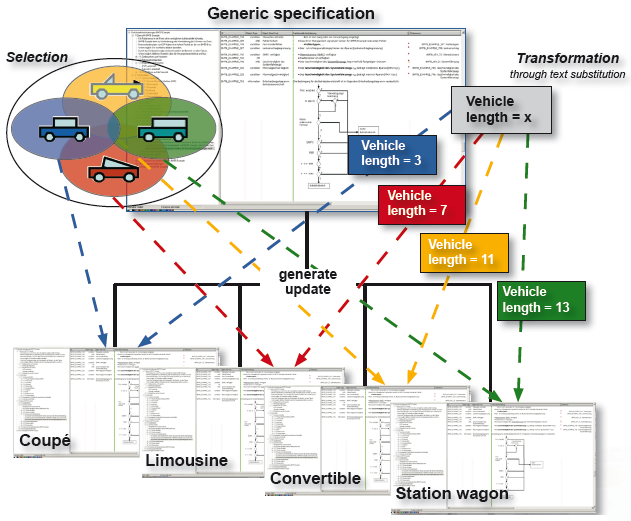
\includegraphics[scale=0.6]{varianten.png}
  		  \caption{Betrachtung von Varianten eines Wagens von der generischen Testspezifikation zur variantenspezifische Testspezifikation aus \cite{VarMan1}}
     \label{doors.bespiel}
  \end{center}
\end{figure}


%#######################################################################################
%#######################################################################################
\newpage
\section{Entwicklungsumgebung und Programmiersprache}
\paragraph{}
TESTONA wurde ursprünglich in der Programmiersprache ...... entwickelt. Mit der Weiterentwicklung wurde das Programm an ...... portiert. Durch den Kauf von Berner \& Mattner in 2008 wurde TESTONA bis zum jetzigen Zeitpunkt auf Java übersetzt und wird weiter mit der Entwicklungsumgebung Eclipse entwickelt.

%#######################################################################################
\subsection{Eclipse}
\paragraph{}
Eclipse ist der Nachfolger von \glqq IMB Visual Age for Java\grqq~ und ist ein quelloffenes Programmierwerkzeug zur Entwicklung verschiedener Art. Ursprünglich war Eclipse als integrierte Entwicklungsumgebung für Java benutzt, aber dank seiner Bedienbarkeit und Erweiterung ist mittlerweile für die Entwicklung in verschiedener Programmiersprachen bekannt (C/C++ und PHP, unter anderen). Die am 25 Juni 2014 veröffentliche Version \glqq Luna\grqq~ (Eclipse 4.4) ist die aktuellste Stand der Software. \\

Mit Eclipse 3.0 hat sich die Grundarchitektur von Eclipse geändert. Seit diesem Zeitpunkt ist Eclipse nur ein Kern, der einzelne Plug-ins lädt. Jedes Plug-in stellt eine oder verschiedene Funktionalitäten zur Verfügung. Darauf aufbauend existiert die \glqq Rich Client Platform\grqq~ (RCP). Diese ermöglicht Entwicklern Anwendungen zu programmieren, die auf das Eclipse Framework aufbauen, aber unabhängig von der Eclipse IDE ist\cite{EclipseRCP} \cite{Eclipse}. Dies ist einer der Hauptgründe warum TESTONA zu Java und Eclipse migriert wurde. Durch die RCP können verschiedene Programmversionen (Light, Express, Professional, Enterprise) besser verwaltet werden. Durch die RCP Architektur können auch verschiedene Funktionalitäten voneinander getrennt werden. Das hilft bei der Weiterentwicklung sowie bei der Pflege des Programms, da mehrere Programmieren gleichzeitig an verschiedenen Plug-ins arbeiten können.\\



%#######################################################################################
\subsection{Plug-ins}
\paragraph{}
Ein Plug-in ist die kleinste ausführbare Softwarekomponente für Eclipse. Um eine Anwedung mit Eclipse RCP zu schreiben, werden mindestens diese drei Plug-ins benötigt:
\begin{itemize}
\item Eclipse Core Plattform: steuert den Lebenszyklus der Eclipse Anwendung
\item Stardard Widget Toolkit: Programmierbibliothek zur Erstellung grafischen Oberflächen
\item JFace: User Interface Toolkit für komplexeren Widgets
\end{itemize}

Weitere Plug-Ins, von der Eclipse Foundation implementiert, stehen den Programmierern zur Verfügung und unter \textit{marketplace.eclipse.org} können auch von Privatentwickler programmierte Plug-Ins heruntergeladen werden. \cite{Eclipse}\\

Plug-ins beinhalten den Java-Code der, wie gewöhnlich, in verschiedene Pakete und Klassen strukturiert werden kann. Sinnvoll ist, dass jedes Plug-in eine Funktionalität des gesamtes Programms repräsentiert, wie zum Beispiel, Variantenmanagement oder Autosave.\\

Testona besteht momentan aus 129 verschiedene Plug-ins, wo jedes Plug-in eine bestimmte Funktion oder Feature des Programms implementiert. Zum Beispiel gibt es für jede Version (Light, Express, Professional und Enterprise) von TESTONA ein Plug-in wo die nötige Plug-ins für die jeweilige Version geladen werden.\\

Ein Plug-in besteht in der Regel aus folgende Einheiten:

\begin{itemize}
\item \textbf{JRE System Library:} beinhaltet alle Systembibliotheken von der Java Runtime Enviroment, dass der jeweilige Plug-in benötigt
\item \textbf{Plug-in Dependencies:} schließt die Abhängigkeiten des Plug-ins mit der Eclipse Umgebung und andere implementierte Plug-ins ein
\item \textbf{src:} bezieht die Pakete und Java-Klassen ein
\item \textbf{icons:} hier befinden sich die Bilderdateien (.gif, .png, etc) die in den Klassen für die Benutzeroberfläche  aufgerufen werden
\item \textbf{META-INF:} gibt eine Übersicht aller Einstellungen des Plug-ins, sowie die Möglichkeit diese über eine graphische Oberfläche zu bearbeiten
\item \textbf{build.properties:} beinhaltet die Einstellungen für das Compilieren des Plug-in. Es kann auch über die META-INF Datei bearbeitet werden.
\item \textbf{plugin.xml:} hier werden die nötige Erweiterungen für das Plug-in definiert. Es ist möglich direkt die \textit{xml} Datei zu bearbeiten, oder die META-INF Oberfläche benutzen.
\end{itemize}

Ein Plug-in kann durchaus mehrere Einheiten oder Elemente beinhalten, wie zum Beispiel weitere \textit{resource} Ordner oder ein Dokumentationsordner mit wichtigen Dokumenten zum Plug-in.
%#######################################################################################
\subsection{Standard Widget Toolkit (SWT)}
\paragraph{}
SWT ist eine seit 2001 von IBM Programmierbibliothek für die Programmierung grafischen Oberflächen unter Java. Die Bibliothek benutzt, im Gegensatz zu Swing\footnote{Programmierschnittstelle und Grafikbibliothek für Java zum programmieren von grafischen Benutzeroberflächen.}, die nativen grafischen Elemente des jeweiligen Betriebssystems und ermöglicht die Erstellung von Anwendungen, die optisch ähnlich wie die nativen Anwendung des Betriebssystems aussehen. Durch die Verwendung der nativen grafischen Elemente, kann das Toolkit sofort Änderungen in das \glqq look and feel\grqq~ des Betriebssystems in der Anwendung aktualisieren und behaltet ein konstantes Programmiermodel in alle Plattformen.
\cite{EclipseSWT}\\

SWT beinhaltet sehr viele komplexe Eigenschaften, aber um eine robuste und benutzbare Anwendung zur Programmieren sind nur die Grundkenntnissen nötig. Eine typische SWT Anwendung hat folgende Struktur:

\begin{itemize}
\item Ein \textit{Display} deklarieren, dieser Repräsentiert die SWT Modus
\item Erstellen eines \textit{Shell}, welche als Hauptfenster dient
\item Erzeugung eines Widgets
\item Initialisierung der Widgetparameter
\item Öffnen des Fensters
\item Starten der Event-Schleife bis eine Abbruchbedingung erfüllt wird (Schließen des Fenster vom Benutzer)
\item Entsorgen des Displays
\end{itemize}

\begin{lstlisting}[caption={Beispiel einer SWT Anwendung}, captionpos=b]
   public static void main (String[] args) {
      Display display = new Display();
      Shell shell = new Shell(display);
      Label label = new Label(shell, SWT.CENTER);
      label.setText("Hello_world");
      label.setBounds(shell.getClientArea());
      shell.open();
      while (!shell.isDisposed()) {
         if (!display.readAndDispatch())
         		display.sleep();
      }
      display.dispose();
   }
\end{lstlisting}

%#######################################################################################
\subsection{JFace}
\paragraph{}
JFace ist ein User Interface Toolkit, dass auf die von SWT gelieferten Basiskomponenten setzt und stellt die Abstraktionsschicht für den Zugriff auf die Komponenten bereit. Es beinhaltet Klassen zur Handhabung gemeinsame Programmieraufgaben, wie zum Beispiel:


\begin{itemize}
\item Viewers: Verbindung von GUI-Elementen zum Datenmodell
\item Actions: definiert Benutzeraktionen und spezifiziert wo diese zur Verfügung stehen
\item Bilder und Fonts: gemeinsame Muster für den Umgang mit Bilder und Fonts
\item Dialoge und Wizards: Framework für komplexere Interaktionen mit dem Benutzer
\item Feldassistent: Klassen die Hilfe an den Benutzer anbieten für richtige Inhaltsauswahl bei Dialoge oder Formulare
\end{itemize}


SWT ist komplett unabhängig von JFace (und Plattform Code), aber JFace wurde konzipiert um SWT zu unterstützen bei allgemeine Benutzerinteraktionen. Eclipse ist wohl das bekannteste Programm das JFace benutzt.\cite{EclipseHelp}